\section{System Analysis: architectural components}
\label{sec:analysis_components}
In this section, we present our investigation into the architecture of the MINA framework. The main focus is to comprehend the structure of the architecture, the dependencies between components and their responsibilities. 
\subsection{Analysis steps}
For conducting this analysis, we investigate the source code \cite{mina-github}, the API documentation \cite{mina-reference} and use the Structure101 tool \cite{structure101} to obtain a clear view of the architecture.\\\\
The first step is importing the MINA project intro Structure101. For clarity and aiding reproducibility, we specify the steps:
\begin{enumerate}
    \item Download latest stable version of MINA, for this report we use version 2.1.3.
    \item Install MINA using command \texttt{MVN CLEAN INSTALL -DSKIPTESTS}
    \item Import MINA as a Maven project in Structure101 through the root pom file.
\end{enumerate}
Having the Structure101 project, we analyze the architecture at a high-level of abstraction; we show how the packages interact and if any patterns are captured by the high-level architecture. This information is presented in section \ref{sec:archi_overview}.\\\\
Following the general overview, each package is individually analysed in section \ref{sec:component_analysis}. For this analysis, we consider the following aspects:
\begin{itemize}
    \item Initial structure of the package
    \item If necessary (i.e. tangles are present), our restructuring of the package
    \item Dependencies and dependents
    \item Inner dependencies
    \item Components and responsibility
    \item Identified patterns
    
\end{itemize}
Finally, we consider one use case of MINA and analyse it from an architectural point of view: how do the architecturally components interact with each other in order to fulfill the functionality of the use case? The use case presents the construction of a MINA server. We will also present the corresponding JAVA implementation.


\subsection{High-level overview of the architecture}
\label{sec:archi_overview}
An account of the high-level architecture structure is presented in figure \ref{fig:packages_structure}; we identify 9 main structural modules:
\begin{enumerate}
    \item \texttt{mina-integration-jmx}: supports JMX integration for managing and monitoring MINA applications.
    \item \texttt{mina-integration-xbean}
    \item \texttt{mina-integration-ognl}
    \item \texttt{mina-integration-beans}
    \item \texttt{mina-filter-compression}: the implementation of a \texttt{IOFilter} which compresses all data using \texttt{JZlib}\cite{jzlib}.
    \item \texttt{mina-http}: implementation of \texttt{http} communication using MINA; exposes an API for MINA applications using the \texttt{http} protocol.
    \item \texttt{mina-statemachine}: offers support for complex applications that would like to implement object state-based behaviour; \texttt{mina-statemachine} implements a improved reinterpretation of the State pattern \cite{state_pattern}.
    \item \texttt{mina-transport-apr}: provides support for APR (Apache Portable Runtime)\cite{apr} transport.
    \item \texttt{mina-core}: the core implementation of the MINA framework; offers the basic functionality by exposing an API for the MINA based applications.
    
\end{enumerate}

\begin{figure}[H]
    \centering
    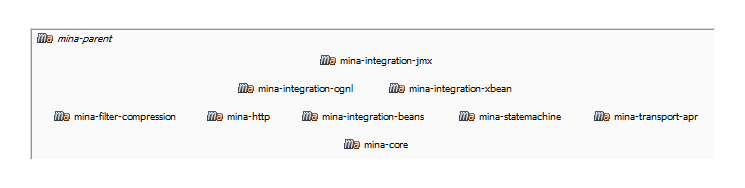
\includegraphics[width=\textwidth]{images/MINA_packages_overview.png}
    \caption{Overview of the package structure of the MINA framework.}
    \label{fig:packages_structure}
\end{figure}

Figure \ref{fig:overview_package_dependencies} in the Appendix shows the overall dependencies between the high-level architectural modules. It is clear that the \texttt{mina-core} module is the back-bone of the framework, the rest of the packages directly or indirectly being dependent on this module (i.e. dependencies flow from top to bottom). Another noticeable aspect is the dependencies between the integration packages, therefore we propose the following restructuring shown in figure \ref{fig:packages_restructure}.

\begin{figure}[H]
    \centering
    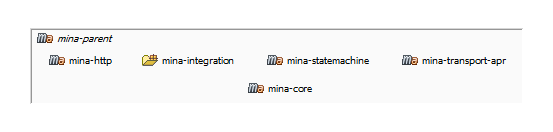
\includegraphics[width=\textwidth]{images/MINA_overview_restructured.png}
    \caption{Overview of the restructured packages of the MINA framework.}
    \label{fig:packages_restructure}
\end{figure}

After the proposed restructuring, the responsibilities of the main modules can be traced as follows, presented in order of importance:
\begin{enumerate}
    \item Implementation of API exposing core functionality of the MINA framework: \texttt{mina-core}
    \item Performance optimization: \texttt{mina-transport-apr}
    \item Additional or advanced functionality which extends the core:  \texttt{mina-http}, \texttt{mina-statemachine}
    \item Third-party integration: \texttt{mina-integration}
\end{enumerate}
In this report, we will emphasize the investigation of the core architecture, in other words, we will focus predominantly on the \texttt{mina-core} module. We expect this module to follow the architectural schema presented in figure \ref{fig:architecture}, since it captures the underlying structure of MINA based applications. This entails that the core module implements the transport layer (i.e. connection to the remote peer as presented in figure \ref{fig:architecture}), the IO service layer, the filters (i.e. IOFilterChain layer in \ref{fig:architecture})  which process the IO and the business logic layer (i.e. IOHandler in figure  \ref{fig:architecture}, a this level the user is able to implement their own logic), all of these components being presided by a session. Keeping in mind the goal of the report at hand, we can already guess the usage of the Layers pattern \cite{archi_patterns}. \\\\
Other remarks regarding the high-level architecture related to the proposed restructuring. Our decision of clustering the integration packages is based on the top-down dependencies between the integration packages as shown in figure \ref{fig:dependencies_integration} in the Appendix, as well as on their serving a common purpose: integration with a third-party entity. The \texttt{mina-filter-compression} has been moved to the core module and grouped together with the useful filter implementations provided by MINA. For the case of the remaining modules that provide additional functionality, we decided to keep the structure proposed by the MINA development team since they serve different purposes and they create more dependencies if included in the core. Their only commonality is that they have been added to extend or optimize the core functionality. Their addition is also fairly new, they have been introduced in version 2.0 (for reference, we analyze Mina version 2.1.3).

\subsection{Component analysis}
\label{sec:component_analysis}
\subsubsection{MINA core}
\textsc{Initial structure}: Appendix, figures \ref{fig:mina_core_initial}, \ref{fig:mina_core_initial_detailed}, \ref{fig:mina_core_core_initial}.  \\
\textsc{Issues and restructuring}: In the initial dependency diagram (i.e. figure \ref{fig:mina_core_dependencies_initial} in the Appendix), cyclic dependencies are marked in red. With the restructuring, we attempted to overcome this problem. However, the nature of the code did not allow for this dependencies to be eliminated. We have, nonetheless, isolated the tangles and reduced the `tangle percentage' from 75\% to 45\%. Diagrams after restructuring are presented in the Appendix, figures \ref{fig:mina_core_restructured}, \ref{fig:mina_core_core_restructured}.\\
\textsc{Dependencies}: None \\
\textsc{Dependents}: All the other modules\\
\textsc{Inner dependencies}: Appendix, figure \ref{fig:mina_core_dependencies_restructured} shows inner dependencies after restructuring.\\
\textsc{Overall responsibility and scope}: This module represents the back-bone of the framework; it spans the base elements that provide support for creating applications using MINA; all other extensions in functionality, integrations or optimizations are highly reliant on this core. Apart from supporting the basic implementation of MINA based client-server applications, it provides useful implementations of IO processing filters, IO handlers and support for the development of MINA based proxy servers.\\
\textsc{Components}: the components are listed as presented in after the restructuring of the architecture:
\begin{enumerate}
    \item \texttt{mina-core-core}: main component of the module, follows the architecture presented in figure \ref{fig:architecture}; it comprises of the crucial components which provide the core functionality of the MINA framework, each components is described in detail in terms of their responsibilities.
        \begin{enumerate}
            \item \texttt{mina-core-core-service}: the most important part of the MINA architecture, it provides crucial IO services and manages the communication sessions with the remote peers. The main responsibilities are managing communication  (i.e. transmits data both ways reads \& writes), listening for \texttt{IOEvent}s, managing \texttt{IOSession}s (creation and deletion, detecting idleness), invoking the \texttt{IOHandler} upon certain events (e.g. messaged received), managing filter chain creation. The \texttt{IOService} interface is implemented by two core classes which provide the desired client-server implementation supported by the framework: \texttt{IOAcceptor}, the server side, and \texttt{IOConnector}, the client side. An overview of all the responsibilities of this module is shown in figure \ref{fig:service_responisbilities}, in the Appendix.
            \item \texttt{mina-core-core-session}: an \texttt{IOSession} represents a client-server connection (i.e. whenever a client connection is established, a new session is created); a session has a \texttt{IOSessionConfig} (e.g. sending/receiving buffer size, idle time etc.) and some user set \texttt{IOSessionAttribute}s (i.e. user defined data that must be persist during the session life-time, this is store in a dedicated \texttt{IOSessionDataStruct} for each session). The \texttt{SessionState} represents the state of the session (see figure \ref{fig:session_lifecycle} in the Appendix). Each session is correlated with a filter chain, all in-going or out-going data is processed  by the chain; moreover, the session is associated with an \textt{IOHandler} which is the communication point with the actual application (it implements the business logic based on the messages/events received). The handler will dispatch the messages received from the session, as well as responding by requesting writes in return. The session handles read/write requests via the \texttt{IOProcessor} which performs the actual IO.
            \item \texttt{mina-core-core-IOEvent}: defines an \texttt{IOEvent}, their types and filter events.
            \item \texttt{mina-core-core-IOFilter}: basic implementation of the \texttt{IOFilter} and \texttt{IOFilterChains}; using the \textit{Adapter} pattern, supports the creation of individual filters or chained filters using a customizable chain filter builder; a filter chain filters all IO events and requests between \texttt{IOService} and \texttt{IOHandler}.
        \end{enumerate}
    \item \texttt{mina-core-proxy}: while \textt{mina-core-core} provides the resources for implementing client-server applications, it provides the support for writing a MINA based proxy server; the proxy module follows the same architecture, providing specific proxy functionality for handlers, filters and sessions which complement the core \textt{IOService}.
    \item \texttt{mina-core-transport}: offers support for several transport types for MINA based applications
        \begin{enumerate}
            \item \texttt{mina-core-transport-socket}: TCP \& UDP implement based on NIO Java API, extended with support for active polling strategies (e.g. NIO select call strategy)
            \item \texttt{mina-core-transport-vmpipe}: in-VM pipe communication (removes overhead of encoding/decoding transmitted data when communication occurs within the same virtual machine).
        \end{enumerate} 
    \item \texttt{mina-core-handler}: useful implementations for \texttt{IOHandler}s
        \begin{enumerate}
            \item \texttt{mina-core-handler-chain}: offers support for implementing sequentially layered protocols via the \textit{Chain of Responsibility pattern}.
            \item \texttt{mina-core-handler-demux}: supports implementation of complex protocols by handling the received data by multiple sub-handlers.
            \item \texttt{mina-core-handler-stream}: a handler adapted for data streams.
            \item \texttt{mina-core-handler-multiton}: enables the creation of one handler per session (as opposed to a handler managing multiple session) via the \textit{Multiton pattern}.
        \end{enumerate}
    \item \texttt{mina-core-IOFilterType}: various useful IOFilter implementations (e.g. logging filter which logs all session communication events, for example "idle session", "messaged received" etc; keep alive filter which offers the ability to keep the connection alive even if data is not being transmitted)
        \begin{enumerate}
            \item \texttt{mina-core-IOFilterTypes-codec}: filter implementations which offer support for protocol development using the codec concept (i.e. a pair of coder/decoder for encoding/decoding specific types of data). 
        \end{enumerate}
    \item \texttt{mina-core-util}: miscellaneous classes used by the entire module, including a custom buffer implementation which replaces the NIO ByteBuffer.
\end{enumerate}
\textsc{Identified patterns}: Chain of Responsibility, Multiton, Adapter, Codec concept.

\subsubsection{MINA integration}
\textsc{Initial structure}: Appendix, figures \ref{fig:jmx_integration}, \ref{fig:ognl_integration}, \ref{fig:xbean_integration}, \ref{fig:beans_integration} \\
\textsc{Issues and restructuring}: No cyclic dependencies\\
\textsc{Dependencies}: \texttt{mina-core}\\
\textsc{Dependents}: None\\
\textsc{Inner dependencies}: Appendix, figure \ref{fig:dependencies_integration}\\
\textsc{Overall responsibility and scope}: Integration with JMX for application management which is built on top of JavaBeans and OGNL integration.\\
\textsc{Components}:
\begin{enumerate}
    \item \texttt{mina-integration-beans}: supports integration of JavaBeans; it implements the \texttt{PropertyEditor} class in order to create convertor classes which transform string objects into various other predefined Java classes (e.g. strings to sets, strings to patterns, strings to files).
    \item \texttt{mina-integration-ognl}: supports integration with the OGNL (Object-Graph Navigation Language) for tasks like finding \texttt{IOSession}s that match a certain OGNL expression or defining OGNL property accessors for IO filters, services and sessions.
    \item \texttt{mine-integration-xbean}: miscellaneous classes mainly adapting the JavaBeans integration with the rest of MINA. 
    \item \texttt{mina-integration-jmx}: supports integration with JMX (Java Management Extensions); it offers the possibility to manage \texttt{IOService}s and \textt{IOSession}s. As per figure \ref{fig:dependencies_integration} in the Appendix, the JMX integration it relies on the achieved integrations described above.
\end{enumerate}\\
\textsc{Identified patterns}: None, possibly a Factory pattern.

\subsubsection{MINA state machine}
\textsc{Initial structure}: Appendix, figures \ref{fig:statemachine_initial}, \ref{fig:statemachine_initial_dependencies}.\\
\textsc{Issues and restructuring}: Cyclic dependencies between the state and transition; for the restructuring, we only reorganized the package, however we could not compensate for the dependency; see Appendix, figures \ref{fig:statemachine_restructured}. \\
\textsc{Dependencies}: \texttt{mina-core}\\
\textsc{Dependents}: None\\
\textsc{Inner dependencies}: Appendix, figure \ref{fig:statemachine_restructured_dependencies} shows inner dependencies after restructuring. \\
\textsc{Overall responsibility and scope}: Extends the core functionality of MINA by supporting the implementation of state based applications; MINA \texttt{statemachine} is similar to the \textit{State} pattern and aims at tackling complexity by organizing the application's process flow into states and transitions. An example is presented in the Appendix, figure \ref{fig:statemachine_example}. We will use this example further on to explain the components of this package. \\
\textsc{Components}: 
\begin{enumerate}
    \item \texttt{State}: a class that implements the state which corresponds with the ellipses (i.e. 'playing', 'pausing') in figure \ref{fig:statemachine_example} in the Appendix. 
    \item \texttt{transition}: implements the transition between \texttt{State}s; a \texttt{Transition} reacts or accepts an \texttt{Event}; upon processing the event, a \texttt{MethodTransition} is executed, which leads to the next \texttt{State} corresponding to the \texttt{Transition}; sometimes no method is required and the transition then just changes the state (goes to next state).
    \item \texttt{event}: \texttt{Event}s trigger \texttt{Transition}s and correspond to methods to be invoked over the transition. Some examples of events that are related to state changes are IO filter and handler events.
    \item \texttt{annotation}: a \texttt{Transition} requires 3 fields: \texttt{inState}, \texttt{method}, \texttt{nextState}; the \texttt{annotation} module defines several interfaces that create the 'annotation' of various types of transitions; these 'annotations' must be defined as the 'rules' of the state machine and capture all the methods in the machine and when these methods can be invoked (i.e. between which states).
    \item \texttt{StateMachine}: based on the \texttt{Transition} annotations defined (i.e. the 'rules'), a \texttt{StateMachine} object is created using the \textit{Factory} pattern. The \texttt{StateMachine} can be seen as a collection of 'rules', however it has no knowledge of the implementation of the transition methods. For this purpose, a \texttt{StateMachineProxyBuilder} is used; this correlates the 'rules' to the actual 'methods'.
    \item{context}: support state awareness; the \texttt{StateContext} holds the current state of the machine; the \texttt{StateContextLookup} gives the current state.
    \item{StateMachineExceptions}: custom exceptions used within the scope of the state machine implementation.
\end{enumerate}
\textsc{Walkthrough}: For this specific module, we present a step-by-step walkthrough of the interaction between components in order to offer a clearer account of the functionality of this module:
\begin{enumerate}
    \item A method is called on the proxy (i.e. \texttt{StateMachineProxyBuilder}).
    \item Search for the current state (i.e. \texttt{StateContext} via  \texttt{StateContextLookup})
    \item Convert the method into an event (i.e. \texttt{Event}s corresponds to methods defined in the state machine)
    \item Invoke the state machine on the event (i.e. the \texttt{StateMachine} will handle the \texttt{Event} by looping through all the defined \texttt{Transition}s that accept the \texttt{Event}; the \texttt{Event} also contains a reference to the current \texttt{StateContext}; match the correct \texttt{Transition})
    \item Execute the transition (i.e. update the current \texttt{StateContext} to the \texttt{nextState} of the matched \texttt{Transition})
\end{enumerate}
\textsc{Identified patterns}: State, Factory, Singleton

\subsubsection{MINA HTTP}
%% Haven't done too much research on this
\textsc{Initial structure}: Appendix, figures \ref{fig:http_structure_initial}, \ref{fig:http_dependencies_initial} \\
\textsc{Issues and restructuring}: Restructuring presented in the Appendix, figure \ref{fig:http_structure_restructured} \\
\textsc{Dependencies}: \texttt{mina-core}\\
\textsc{Dependents}: None\\
\textsc{Inner dependencies}: Appendix, figure \ref{fig:http_dependencies_restructured} shows inner dependencies after restructuring. \\
\textsc{Overall responsibility and scope}: supports implementation of MINA based applications which use the HTTP protocol.\\
\textsc{Components}: 
\begin{enumerate}
    \item \texttt{HttpClientCodec} \& \texttt{HttpServerCodec}: using the \textit{codec} concept, defines encoders and decoders for client-server applications communicating over HTTP.
    \item \texttt{DecoderState}: defines the three states of a decoder: waiting for a new request, received the header of the request, received the body of the request.
    \item \texttt{HttpRequestImpl}: basic implementation of a HTTP request.
    \item \texttt{api}: exposes a HTTP API.
    \item \texttt{util}: miscellaneous classes that are used within the scope of the \texttt{http} package.
\end{enumerate}
\textsc{Identified patterns}: Codec mechanism, Client-Server.\\

\subsubsection{MINA transport APR}
%% Haven't done too much research on this
\textsc{Initial structure}: Appendix, figures \ref{fig:apr_structure}.  \\
\textsc{Issues and restructuring}: None \\
\textsc{Dependencies}: \texttt{mina-core}\\
\textsc{Dependents}: None\\
\textsc{Inner dependencies}: Appendix, figure \ref{fig:apr_dependencies}. \\
\textsc{Overall responsibility and scope}: Support for APR (Apache Portable Runtime) transport which ensures superior scalability and performance; allows for better integration with native server technologies. \\
\textsc{Components}: The components follow the structure defined in the \texttt{core} module; the \texttt{IOProcessor} and \texttt{IOSession} have been adapted to implement APR. \\
\textsc{Identified patterns}: None \\


\subsection{Use case analysis: creating a MINA server}
We present the use case of creating a MINA based server. Even though it is a rather simple use case, it captures the core functionality of MINA as a networking framework. With this use case, we intend to show how the core components of MINA interact with each other in order to obtain the server functionality. Apart from presenting the steps that lead to the successful creation of a MINA server, we also show their implementation; the call graphs of the methods used are listed in the Appendix, section \ref{sec:call_graphs}.\\\\
\underline{\textsc{Step 1}}:\\
The core requirement of a server is to accept client connections. This implies that a mechanism for listening to incoming, possible connections is required. This mechanism is dependent on the type of communication between the server and the clients. MINA offers two main possibilities here: either TCP/IP or UDP/IP.\\\\
In this example, we construct a TCP/IP server. We include an \texttt{IOAcceptor} which listens for connections over a \texttt{SocketAcceptor} and is bound to a user defined port:

\begin{verbatim}
    IOAcceptor connectionsAcceptor = new NIOSocketAcceptor();
    // bind the acceptor to a port of value PORT
    connectionsAcceptor.bind( new InetSocketAddress(PORT));
\end{verbatim}

This also implies a connection between the \texttt{transport} and the \texttt{service} packages (see figure \ref{fig:step1}):


% \begin{figure}
%     \centering
%     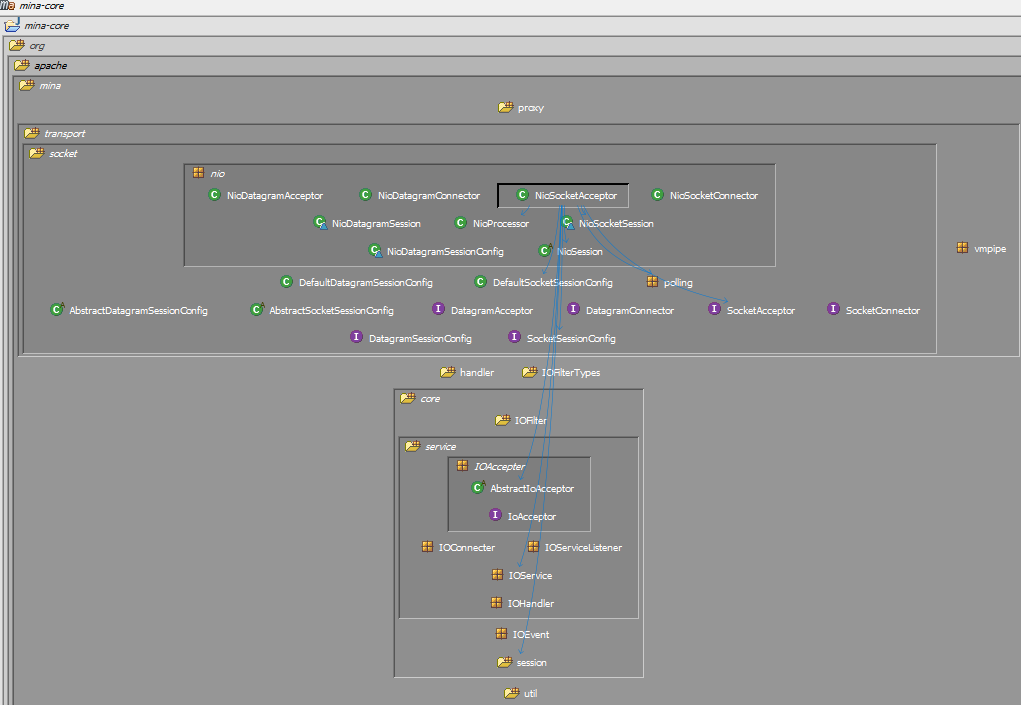
\includegraphics[width=\textwidth]{images/IOacceptor.png}
%     \caption{Architectural implications of step 1 in the server use case.}
%     \label{fig:step1}
% \end{figure}

\underline{\textsc{Step 2}}:\\
The following step is to define a handler, an instance which will react to the communication events between the clients and our server. The responsibility of the handler is to implement the user defined business logic: what actions should be taken when a client connects to the server? or when a message is received?\\\\
The handler needs to be added to the \texttt{connectionsAcceptor}; it will be an user-defined implementation of the \texttt{IOHandlerAdapter} class:

\begin{verbatim}
    // serverHandler extends IOHandlerAdapter
    connectionsAcceptor.setHandler(new serverHandler());
\end{verbatim}

This establishes a connection between packages \texttt{IOAcceptor} and \texttt{IOHandler} via the \texttt{IOHandler} interface.

\underline{\textsc{Step 3}}:\\
Since the server deals with IO communication, MINA offers the possibility of applying filters on the client connections and, therefore, on the inflow/outflow of data. Filters can be chained to obtain the functionality desired by the user.\\\\
Each \texttt{IOAdapter} has a predefined \texttt{DefaultFilterChainBuilder} which creates a corresponding \texttt{FilterChain}; this allows the user to easily add various types of filters to the chain:

\begin{verbatim}
    // adds a new logging filter as the last element of the filter chain
    connectionsAcceptor.getFilterChain().addLast("logging filter", new LoggingFilter());
    /* adds a encoder/decoder protocol filter which transforms message objects 
    *into specific data types
    *TextLineCodecFactory handles text based messages 
    */
    connectionsAcceptor.getFilterChain().addLast("text codec", 
    new ProtocolCodecFilter(new TextLineCodecFactory( Charset.forName( "UTF-8"))));
\end{verbatim}

In this manner, the \texttt{IOService} package is also related to the \texttt{IOFilter} component, which in turn is related to the \texttt{IOFilterTypes} package.

\underline{\textsc{Step 4}}:\\
Whenever a client connection is established with the server, a new session is created by default (more accurately, it becomes active). The acceptor's responsibility is to create and manage this session correspondingly, as well as to notify the handler of the events occurring during the session. This process is part of the inner workings of MINA.\\\\
The user, however, has the option to configure the \textt{IOSession} according to their specifications:

\begin{verbatim}
    // sets the IO buffer size to SIZE
    connectionsAcceptor.getSessionConfig().setReadBufferSize(SIZE);
    // determine acceptable idle time of the connection
    connectionsAcceptor.getSessionConfig().setIdleTime(IdleStatus.BOTH_IDLE, 10);
\end{verbatim}

This directly connects the \texttt{service} and the \texttt{session} packages.





